\reviewexercisesheader{}

% 43 - makeup_exam

\eoce{\qt{Make-up exam\label{makeup_exam}} \videosolution{ahss_eoce_sol-makeup_exam} In a class of 25 students, 24 of them took an exam 
in class and 1 student took a make-up exam the following day. The professor graded the 
first batch of 24 exams and found an average score of 74 points with a standard 
deviation of 8.9 points. The student who took the make-up the following day scored 64 
points on the exam.
\begin{parts}
\item Does the new student's score increase or decrease the average score?
\item What is the new average?
\item Does the new student's score increase or decrease the standard deviation of the 
scores?
\end{parts}
}{}

% 44 - infant_mortality_rel_freq

\eoce{\qt{Infant mortality\label{infant_mortality}} The infant mortality rate is defined as 
the number of infant deaths per 1,000 live births. This rate is often used as an 
indicator of the level of health in a country. The relative frequency histogram below 
shows the distribution of estimated infant death rates for 224 countries for which such 
data were available in 2014. 
\footfullcite{data:ciaFactbook}

\noindent\begin{minipage}[c]{0.43\textwidth}
\begin{parts}
\item Estimate Q1, the median, and Q3 from the histogram.
\item Would you expect the mean of this data set to be smaller or larger than the 
median? Explain your reasoning.
\end{parts} \vfill \
\end{minipage}
\begin{minipage}[c]{0.52\textwidth}
\hfill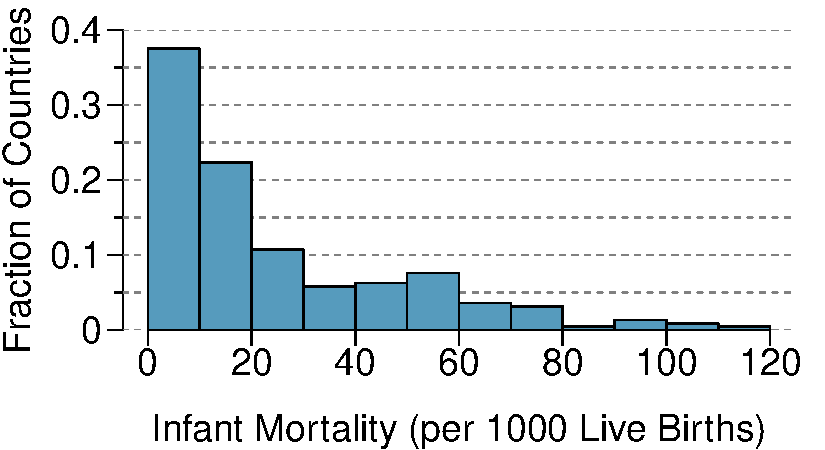
\includegraphics[width = 0.85\textwidth]{ch_summarizing_data/figures/eoce/infant_mortality_rel_freq/infant_mortality_rel_freq_hist.pdf}
\end{minipage}
}{}

% 45 - dist_shape_tv_watchers

\eoce{\qt{TV watchers\label{dist_shape_TV_watchers}} Students in an AP Statistics class 
were asked how many hours of television they watch per week (including online 
streaming). This sample yielded an average of 4.71 hours, with a standard 
deviation of 4.18 hours. Is the distribution of number of hours students watch 
television weekly symmetric? If not, what shape would you expect this distribution 
to have? Explain your reasoning.
}{}

% 46 - new_stat

\eoce{\qt{A new statistic\label{new_stat}} The statistic $\frac{\bar{x}}{median}$ can 
be used as a measure of skewness. Suppose we have a distribution where all 
observations are greater than 0, $x_i > 0$. What is the expected shape of 
the distribution under the following conditions? Explain your reasoning.
\begin{parts}
\item $\frac{\bar{x}}{median} = 1$
\item $\frac{\bar{x}}{median} < 1$
\item $\frac{\bar{x}}{median} > 1$
\end{parts}
}{}

% 47 - oscar_winners

\eoce{\qt{Oscar winners\label{oscar_winners}} The first Oscar awards for best actor 
and best actress were given out in 1929. The histograms below show the age 
distribution for all of the best actor and best actress winners from 1929 to 
2018. Summary statistics for these distributions are also provided. Compare the 
distributions of ages of best actor and actress winners.\footfullcite{data:oscars} \\
\begin{minipage}[c]{0.72\textwidth}
\begin{center}
\tabspecial{tableau-oscar-winner}{
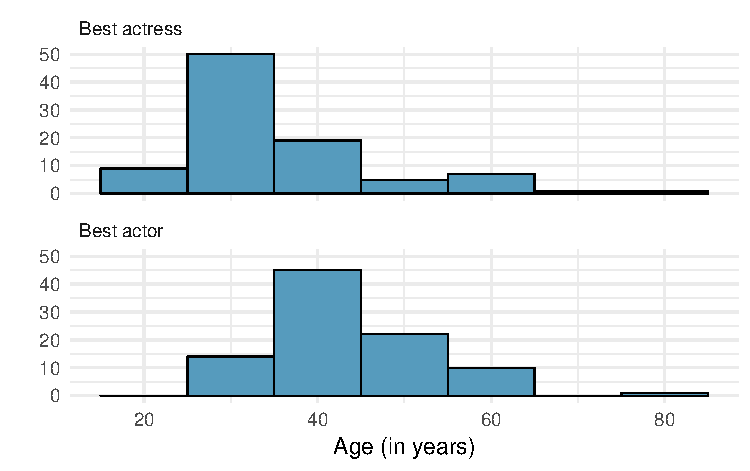
\includegraphics[width=0.95\textwidth]{ch_summarizing_data/figures/eoce/oscar_winners/oscars_winners_hist.pdf}}
\end{center}
\end{minipage}
\begin{minipage}[c]{0.27\textwidth}
{\small
\begin{tabular}{l c}
\hline
        & Best Actress  \\
\hline
Mean    & 36.2      \\
SD      & 11.9      \\
n       & 92        \\  
        & \\
        & \\
        & \\
        & \\
        & \\
\hline
        & Best Actor \\
\hline
Mean    & 43.8 \\
SD      & 8.83 \\
n       & 92
\end{tabular}
}
\end{minipage}
}{}

% 48 - dist_shape_exam_scores

\eoce{\qt{Exam scores\label{dist_shape_exam_scores}} The average on a history exam 
(scored out of 100 points) was 85, with a standard deviation of 15. Is the 
distribution of the scores on this exam symmetric? If not, what shape would 
you expect this distribution to have? Explain your reasoning.
}{}

% 49 - stats_scores_box

\eoce{\qt{Stats scores\label{stats_scores_box}} Below are the final exam scores of twenty 
introductory statistics students.
\begin{center}
57, 66, 69, 71, 72, 73, 74, 77, 78, 78, 79, 79, 81, 81, 82, 83, 83, 88, 89, 94
\end{center}
Create a box plot of the distribution of these scores. The five number summary provided below may be useful.
\begin{center}
\renewcommand\arraystretch{1.5}
\begin{tabular}{ccccc}
Min & Q1    & Q2 (Median)   & Q3    & Max \\
\hline
57  & 72.5  & 78.5          & 82.5  & 94 \\
\end{tabular}
\end{center}
}{}

% 50 - marathon_winners

\eoce{\qt{Marathon winners\label{marathon_winners}} The histogram and box plots below show the distribution of finishing times for male and female winners of the New York Marathon between 1970 and 1999.
\begin{center}
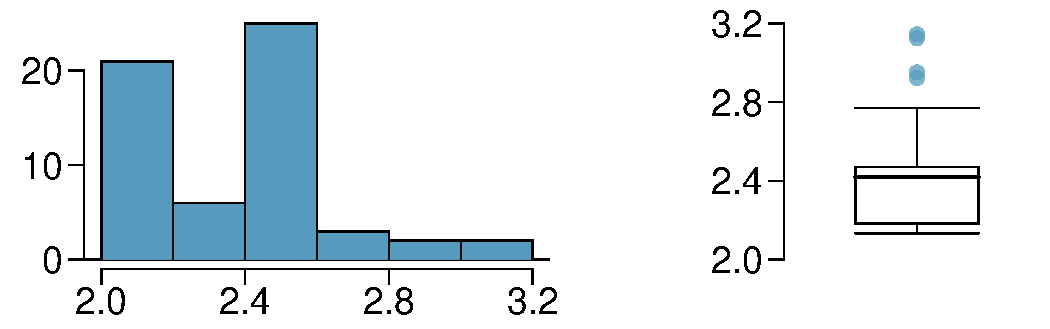
\includegraphics[width=0.56\textwidth]{ch_summarizing_data/figures/eoce/marathon_winners/marathon_winners_hist_box.pdf}
\end{center}
\begin{parts}
\item What features of the distribution are apparent in the histogram and not the box plot? What features are apparent in the box plot but not in the histogram?
\item What may be the reason for the bimodal distribution? Explain.
\item Compare the distribution of marathon times for men and women based on the box plot shown below.
\begin{center}
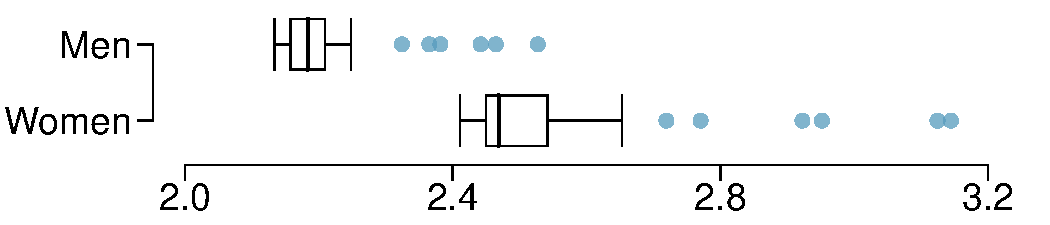
\includegraphics[width=0.56\textwidth]{ch_summarizing_data/figures/eoce/marathon_winners/marathon_winners_gender_box.pdf}
\end{center}
\item The time series plot shown below is another way to look at these data. Describe what is visible in this plot but not in the others.
\end{parts}
\begin{center}
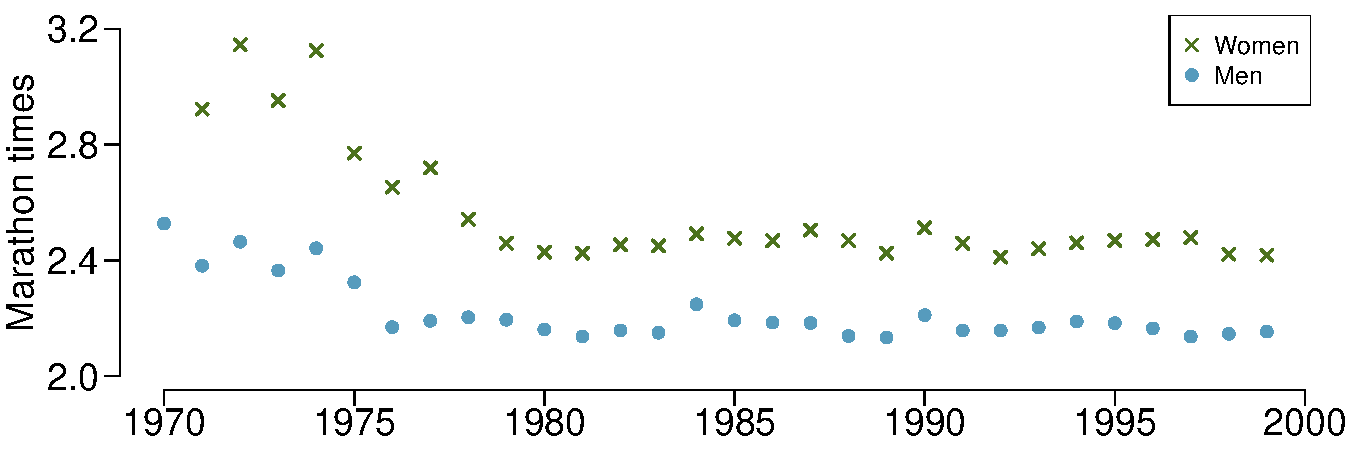
\includegraphics[width=0.6\textwidth]{ch_summarizing_data/figures/eoce/marathon_winners/marathon_winners_time_series.pdf} \\
\end{center}
}{}

% 51 - birth_weight

\eoce{\qt{Birth weight\label{birth_weight}}
In a large study of birth weight of newborns, the weights of 23,419 newborn boys were recorded. The distribution of weights was approximately normal with a mean of 7.44 lbs (3376 grams) and a standard deviation of 1.33 lbs (603 grams). The government classifies a newborn as having low birth weight if the weight is less than 5.5 pounds.\footnote{\oiRedirect{textbook-birthweight_for_Scottish_singleton_births}{www.biomedcentral.com/1471-2393/8/5}}
\begin{parts}
\item What percent of these newborns had a low birth weight?
\item Approximately what percent of these babies weighed greater than 10 pounds?
\item Approximately \emph{how many} of these newborns weighed greater than 10 pounds?
\item How much would a newborn have to weigh in order to be at the 90th percentile among this group?
\end{parts}
}{}

% 52 - auto_insurance_premiums

\eoce{\qt{Auto insurance premiums\label{auto_insurance_premiums}} Suppose a 
newspaper article states that the distribution of auto insurance premiums for 
residents of California is approximately normal with a mean of \$1,650. The 
article also states that 25\% of California residents pay more than \$1,800. 
\begin{parts}
\item What is the Z-score that corresponds to the top 25\% (or the $75^{th}$ 
percentile) of the standard normal distribution?
\item What is the mean insurance cost? What is the cutoff for the 75th 
percentile?
\item Identify the standard deviation of insurance premiums in California.
\end{parts}
}{}

% 53 - speeding_i5_intro

\eoce{\qt{Speeding on the I-5, Part I\label{speeding_i5_intro}} The distribution of 
passenger vehicle speeds traveling on the Interstate 5 Freeway (I-5) in 
California is nearly normal with a mean of 72.6 miles/hour and a standard 
deviation of 4.78 miles/hour.\footfullcite{Johnson+Murray:2010}
\begin{parts}
\item What percent of passenger vehicles travel slower than 80 miles/hour?
\item What percent of passenger vehicles travel between 60 and 80 miles/hour?
\item How fast do the fastest 5\% of passenger vehicles travel?
\item The speed limit on this stretch of the I-5 is 70 miles/hour. 
Approximate what percentage of the passenger vehicles travel above the speed 
limit on this stretch of the I-5.
\end{parts}
}{}

% 54 - heights_10_yrs

\eoce{\qt{Heights of 10 year olds, Part I\label{heights_10_yrs}}
Heights of 10 year olds, regardless of gender, closely follow
a normal distribution with mean 55 inches and standard deviation
6~inches.
\begin{parts}
\item
    What is the probability that a randomly chosen 10 year old
    is shorter than 48 inches?
\item
    What is the probability that a randomly chosen 10 year old
    is between 60 and 65 inches?
\item
    If the tallest 10\% of the class is considered
    ``very tall'',
    what is the height cutoff for ``very tall"?
\end{parts}
}{}
